\chapter{How to Use a Journal}

This lecture begins at the point where enthusiasm usually fails: the listener buys a journal, opens it, and is confronted by blank pages. From there the lecture develops a practical mathematics of self-management. We begin with the object itself, move to writing as a device for clarification and problem solving, widen to the capture and organization of ideas, and end with review, communication, imagination, and legacy. The formulas in this chapter are therefore heuristic rather than scientific; they compress the lecture's method into a set of usable rules.

\paragraph{Heuristic status.}
The equations in this chapter should be read as disciplined summaries of the lecture's procedure. They are not formal laws of psychology or economics. Their role is to preserve the structure of the argument: how writing separates us from confusion, how review turns storage into knowledge, and how a journal becomes a bridge from intention to action.

\section{Blank Pages, Ownership, and the Habit of Beginning}

The opening tension is simple. People hear a persuasive talk, decide to keep a journal, and then discover that inspiration is easier than use. Instead of answers, the blank page seems to produce a flood of questions: what shall we write, how often, about what, and in what sort of book? The lecture answers by refusing to separate philosophy from instrument. Before the journal becomes a device for thought, it must become an object we are willing to carry, open, and use.

The first claim is that the journal is \emph{your} book. Size, paper, lines or blank pages, binding, and portability are therefore not decorative details. They enter into the practical problem of use. The lecture even pauses over such apparently minor features as the color of the cover, the feel of the paper, and the physical pleasure of holding the book. The point is not luxury for its own sake. The point is that use depends on felt suitability.

\begin{equation}
\operatorname{Use}(J)\propto \operatorname{Feel}(J)
\end{equation}

Here \(J\) denotes the journal considered as a working object. The relation is not numerical, but it is explicit in the lecture: the use of anything received is in direct proportion to how it makes us feel when we use it.

A cautious standard reconstruction of the same thought is
\begin{equation}
\operatorname{Effectiveness}(J)=f(\text{fit},\text{comfort},\text{portability},\text{habit}).
\end{equation}

This section of the lecture also makes a second point, and it is easy to lose if we summarize too quickly. Systems change. Loose-leaf binders, notebooks, hardbound volumes, lined pages, blank pages: each may serve a need for a time. Flexibility is therefore part of the method. But flexibility is not indecision. At the beginning, one thing matters more than refinement:
\[
\text{first success}=\text{the formation of the journal habit}.
\]

The lecture's first discipline is not daily volume. It is simpler than that and, in practice, harder: always have the journal with us.

\section{What Goes into a Journal? Writing as Clarification and Problem Solving}

The lecture then announces a pivot. Buying the journal is easy; filling it is the difficulty. The question is no longer what form the book should take, but what function it should perform.

\subsection{Question \& Answer}

The natural question is: \emph{What should go into a journal if it is to have meaning and value in life?}

The answer is not first a list of topics. The answer is to understand what the journal does. Once we see why we write, what we write becomes much less mysterious. The lecture's first major function is that writing helps us figure things out: life, people, business dilemmas, and ourselves.

A compact reconstruction of the lecture's central process is
\begin{equation}
\text{vague problem}\rightarrow \text{written description}\rightarrow \text{factual picture}\rightarrow \text{actionable adjustment}.
\end{equation}

This is immediately followed by the lecture's strongest process claim:
\begin{equation}
\text{write problem}\rightarrow \text{discover ways of making it right}.
\end{equation}

The reasoning is that writing creates distance. A problem merely carried in the mind tends to mix itself with imagination, fear, hurry, and distortion. A problem written down becomes something we can inspect. The lecture does not treat this as magic in the mystical sense. It treats it as a change of viewpoint.

We can make the lecture's update rule more explicit:
\begin{equation}
\text{mental picture}_{n+1}=R\!\left(\text{written account}_{n}\right),
\end{equation}
where \(R\) denotes rereading or review. The new picture replaces the older distorted one, and once things are seen more nearly as they are, they become more nearly manageable.

\begin{figure}[h]
\centering
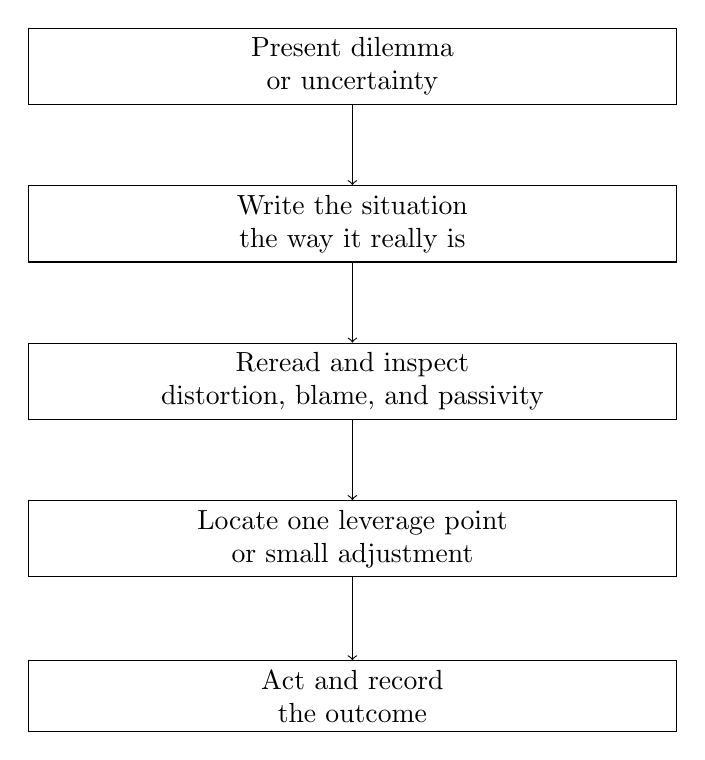
\begin{tikzpicture}
\node[draw, align=center, text width=8cm] (a) at (0,0) {Present dilemma\\or uncertainty};
\node[draw, align=center, text width=8cm] (b) at (0,-2.0) {Write the situation\\the way it really is};
\node[draw, align=center, text width=8cm] (c) at (0,-4.0) {Reread and inspect\\distortion, blame, and passivity};
\node[draw, align=center, text width=8cm] (d) at (0,-6.0) {Locate one leverage point\\or small adjustment};
\node[draw, align=center, text width=8cm] (e) at (0,-8.0) {Act and record\\the outcome};
\draw[->] (a) -- (b);
\draw[->] (b) -- (c);
\draw[->] (c) -- (d);
\draw[->] (d) -- (e);
\end{tikzpicture}
\caption{A transcript-backed journal cycle for the lecture's first function: writing creates enough distance for correction and action.}
\end{figure}

This is why the lecture recommends that one of the first entries may be a current dilemma. We are not told to wait until we have something literary to say. We are told to begin where life is already difficult.

\section{Distortion, Responsibility, and the Weak Point}

Once the problem has been written, the lecture narrows into analysis. What are we to look for in the written account? The sequence is careful and pedagogical. First, distortions. Second, blame. Third, passive hope. Fourth, the weak point in the obstacle.

\paragraph{Worked update rule.}
Let \(P\) be a present problem and let \(W_k(P)\) denote the \(k\)-th revision of its written statement. Then the lecture's method may be organized as
\begin{align}
W_0(P)&=\text{first telling of the problem},\\
W_1(P)&=\text{remove exaggeration or unwarranted optimism},\\
W_2(P)&=\text{remove blame shifted to circumstances or other people},\\
W_3(P)&=\text{remove passive hope and identify one controllable adjustment},\\
O(P)&=\text{record the eventual outcome}.
\end{align}

The force of this scheme is that the statement is refined before the action is chosen. Writing is not the substitute for action; it is the preparation for action.

At the center of this section stands one of the lecture's maxims:
\begin{equation}
\text{things get better when you get better}.
\end{equation}

This is the explicit rejection of the fantasy that circumstances or other people must first change before our own difficulty can be relieved. The lecture is not denying that circumstances matter. It is insisting that passive hope is not a working method.

A second maxim follows immediately:
\begin{equation}
\text{major problem}\approx \text{few minor adjustments in attitude or action plan}.
\end{equation}

This is framed through the David and Goliath image and through the metaphor of the microscope. We are asked to view the problem as a scientist might view an organism on a slide: not as an indistinct mass, but as something with real shape, boundary, and composition. The leverage point need not be large. It needs only to be real.

The lecture then adds a crucial bookkeeping instruction. When the solution or outcome arrives, record it. If the action worked, it is worth preserving. If it failed, it is even more important to preserve, since the most expensive error is not the first one but the repeated one. The journal therefore becomes a memory against recurrence.

\section{Commitment Now and the Capture of Ideas}

At this point the lecture makes a sharp tonal turn. A suggestion may be excellent and still remain useless if it is postponed. The key enemy is the word ``sometime.'' The movement here is from method to discipline.

A compressed form of the warning is
\begin{equation}
\text{intent}\not\Rightarrow \text{accomplishment}.
\end{equation}

The lecture's demand is concrete: if the suggestion is good, do not promise to try it later. Open the journal and write at least one page. Without the discipline to begin, there will not be the discipline to continue.

From this pressure the lecture opens its second major function: the capture of good ideas. A quote, a sermon, a conversation, an observation, a business detail, a personal discovery---each appears and vanishes quickly unless seized at once. The church anecdote is important here because it dramatizes the difference between the serious student and the casual hearer. Others assume they will remember. The student writes.

The central inequalities are straightforward:
\begin{equation}
\text{information captured now}>\text{fragments remembered later},
\end{equation}
and
\begin{equation}
\text{idea on paper}\rightarrow \text{etched more firmly in consciousness}.
\end{equation}

The lecture is explicit that hearing, seeing, or reading something is one thing; taking the time and effort to put it on paper is another. Writing does not merely store the idea. It deepens the idea's hold on consciousness.

This section also introduces a long temporal horizon. The idea we capture today may not yet have a use, but later it may prove to be exactly the piece of intellectual equipment required when opportunity or conflict arrives. The journal is therefore not only a notebook. It is an armory.

\section{From Fragments to Organized Knowledge}

Capture alone is insufficient. The lecture next turns to accumulation and then to organization. Ideas gathered around a theme have a tendency to cohere. The metaphors of snowflakes, snowballs, and the igloo are doing real work here: many tiny elements, once assembled and compressed, form something inhabitable.

A careful transcript-backed compression is
\begin{equation}
\text{snowflakes}\rightarrow \text{blocks}\rightarrow \text{structure},
\end{equation}
and then, more explicitly,
\begin{equation}
\text{good ideas in one area}\rightarrow \text{solid block},\qquad
\text{solid blocks}\rightarrow \text{whole new life}.
\end{equation}

But a block that cannot be found may as well not exist. This is why the lecture turns from collection to indexing. The mind by itself is likened to a cluttered drawer: valuable things are there, but they are irretrievable because they were stored helter-skelter.

The journal is proposed as a logical storage device, and the lecture even gives explicit index-style data:
\begin{align}
\text{Financial Ideas}&\mapsto \{5,53,96,104\},\\
\text{Ideas for Increasing Company Efficiency}&\mapsto \{46,82,111\}.
\end{align}

The examples of three separate journals, three colors of ink, and finally reserved sections within one volume are not side remarks. They show the lecture experimenting toward a practical compromise between purity of classification and ease of use. The final lesson is not that one system is universally best. It is that \emph{some} system is necessary.

The same point may be stated as
\begin{equation}
\text{capture}+\text{organization}+\text{review}\rightarrow \text{practical knowledge}.
\end{equation}

Without organization, even rich capture remains inert. Opportunity appears, knocks, and departs while we search for the key.

\section{Review, Self-Discovery, Events, and Patterns}

The next pivot is marked as a key point in the lecture: journals attain their greatest value when they are reviewed. Writing is only the first half of the operation.

The lecture's own two-stage formula is
\begin{equation}
\text{writing}=\text{capture},\qquad
\text{re-reading}=\text{translation of information into practical knowledge}.
\end{equation}

This rereading has several consequences. First, it makes visible a story of growth. Second, it reveals omission as well as inclusion. Third, it brings events and feelings into relation. Fourth, it lets us see patterns that are invisible at the scale of a single day.

To support this pattern-reading, the lecture recommends recording the date, time, and location of each entry. We may treat this as a coordinate triple
\begin{equation}
M=(\text{date},\text{time},\text{location}).
\end{equation}

That small formal addition matters because it allows a genuine worked example drawn directly from the lecture. A man reviews his journal and finds a recurrent negative pattern. The pattern is indexed not merely by mood but by time.

\paragraph{Worked example: the Wednesday pattern.}
Let the \(n\)-th entry carry metadata \(M_n=(d_n,t_n,\ell_n)\). The lecture's example can be written as
\begin{align}
d_n=\text{Wednesday},\qquad t_n=\text{afternoon or evening}
&\Longrightarrow \text{recurrent self-doubt and discouragement},\\
\text{identify recurring luncheon association}
&\Longrightarrow \text{source of the negative pattern},\\
\text{remove or revise the association}
&\Longrightarrow \text{the pattern weakens or disappears}.
\end{align}

This is a strong example because it shows the journal acting almost experimentally. A suspected cause is proposed, comparison cases are checked, and the influence is isolated.

The lecture then generalizes from patterns to emotional understanding:
\begin{equation}
\text{cause}\rightarrow \text{effect},
\end{equation}
and, more specifically,
\begin{equation}
\text{external event}\rightarrow \text{written description}\rightarrow \text{inner understanding}.
\end{equation}

This connects observation to self-knowledge. The better we describe what goes on around us, the better we understand what goes on within us.

There is also a direct claim about emotional handling that is secure enough to preserve:
\begin{equation}
\text{powerful negative emotion}\xrightarrow{\text{writing}}\text{diminished strength}.
\end{equation}

A nearby line about positive emotions is textually unstable in the transcript, so the safest final statement is the one the lecture immediately clarifies: writing about fear reduces its strength, and capturing excitement can intensify and stabilize it.

\section{Communication, Frequency, and the Inward Decision}

From self-discovery the lecture widens to communication. The journal first gives us a place to speak to ourselves and hear what we are saying. Only then does it become an instrument for dealing more truthfully with others.

A compact form of the claim is
\begin{equation}
\text{clearer self-description}\rightarrow \text{clearer communication with others}.
\end{equation}

The lecture's sequence is important. One writes problems, observations, emotions, and reactions; one then begins asking oneself questions on paper; from that question-and-answer process there comes an increase in self-understanding; and from that increase there comes an outward improvement in expression and listening.

\subsection{Question \& Answer}

At this stage the lecture raises another natural question: \emph{How often should we be writing?}

The answer is deliberately balanced. As often as we wish and as often as we need. But two extremes are rejected: never writing, and constantly writing. The first means participation without capture; the second means capture without participation. The lecture compresses its answer into a useful formula:
\begin{equation}
\text{life}=\text{observation}+\text{action}.
\end{equation}

The journal belongs on the observation side, but not to the exclusion of living. This is why the lecture again stresses carrying the journal more than filling it by compulsion. The habit of availability is primary.

The discussion then returns to agency in its strongest form:
\begin{equation}
\text{decision}+\text{action}\ \text{must come from inside you}.
\end{equation}

No tape, no book, no seminar, and no external encouragement can substitute for this. The anecdote about the nearly five hundred listeners, only a few of whom were actually keeping journals months later, is the lecture's proof that admiration is cheap and discipline is dear.

\section{Imagination, Goals, and Legacy}

The closing movement enlarges the journal once more. It is not only a record of problems, ideas, emotions, and patterns. It is also a place to design life before life is lived. The lecture asks us to become the author of our own life: create imagined circumstances on paper, place ourselves within them, and observe the resulting picture.

The transition from imagination to action is one of the lecture's cleanest constructive sequences:
\begin{equation}
\text{dreams}\rightarrow \text{written goals with priorities and deadlines}\rightarrow \text{detailed plan of action}.
\end{equation}

This is the point at which the journal ceases to be merely archival. It becomes projective. Ideal work, ideal relationship, ideal income, ideal conduct, ideal lifestyle: these are first painted mentally, then written, then broken into steps.

The lecture closes by placing this process inside a much larger horizon. Two quotations appear in equation-like form:
\begin{equation}
\text{conceive}+\text{believe}\Rightarrow \text{achieve},
\end{equation}
and
\begin{equation}
\text{thinketh}\rightarrow \text{becomes}.
\end{equation}

These should be treated as quoted maxims rather than as original formal laws of the lecture. Their function is to reinforce the chapter's final expansion: what is written does not remain merely written. Under belief, commitment, discipline, and desire, it seeks embodiment.

The final pages of the lecture move from personal ambition to inheritance. Journals capture hopes, sorrows, lessons, achievements, disappointments, and the knowledge of a single life. In that sense a journal is not only a private aid. It is a contribution to a shared human heritage. Civilization, on this view, is not inherited automatically; it is learned, earned, gathered, and transmitted. The journal becomes one of the humble instruments by which that transmission occurs.

\section{Summary}

We can now see the lecture as a single chain. The journal is first chosen so that it may be used. It is then used to write a present problem, and writing separates confusion from the self. Analysis removes distortion, blame, and passivity. Ideas are captured before they evaporate, organized before they are lost, and reviewed before they harden into dead storage. Events, feelings, and patterns are tied together. Communication improves because inner description becomes more accurate. Finally, imagination is written into goals, and goals into plans. The lecture thus treats the journal as object, method, memory, mirror, bridge, and design table all at once.